%Secci�n: Introducci�n Ingenier�a de Software

\chapter{Ingenier�a de Software}
\section{Introducci�n}
\subsection{Definici�n}

La \emph{Ingenier�a de Software} es la aplicaci�n de un acercamiento sistem�tico, disciplinado y cuantificable para el desarrollo, operaci�n y mantenimiento de un software.

La Ingenier�a de Software(IS) re�ne conocimientos, herramientas y m�todos para definir requerimientos de software y realizar dise�o, construcci�n, testing y mantenimiento de software.

\subsubsection{Objetivo:} Se ocupa de construir un producto de software de buena calidad, lidiando con m�ltiples restricciones (tiempo, presupuesto, requerimientos, etc)

\subsubsection{Problem�ticas:}
\begin{itemize}
	\item Lidiar con la escala y complejidad de sistemas de software
	\item Identificar que significa buena calidad
	\item Disciplina joven, v�ctima de su propio �xito
\end{itemize}

\section{Ciclo de Vida de Desarrollo de Software}

\subsection{Modelo Cascada (Royce, 1970)}

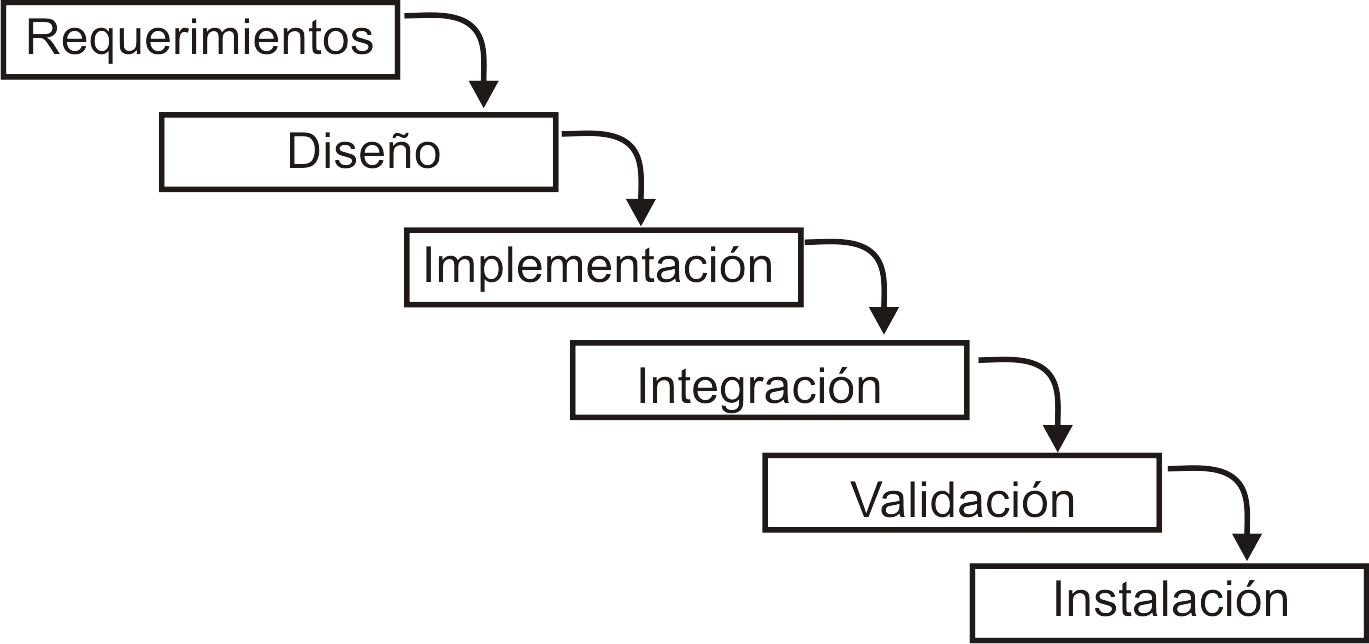
\includegraphics[width = 0.9\textwidth]{Graficos/ModeloCascada.png}

\subsection{Modelo V}

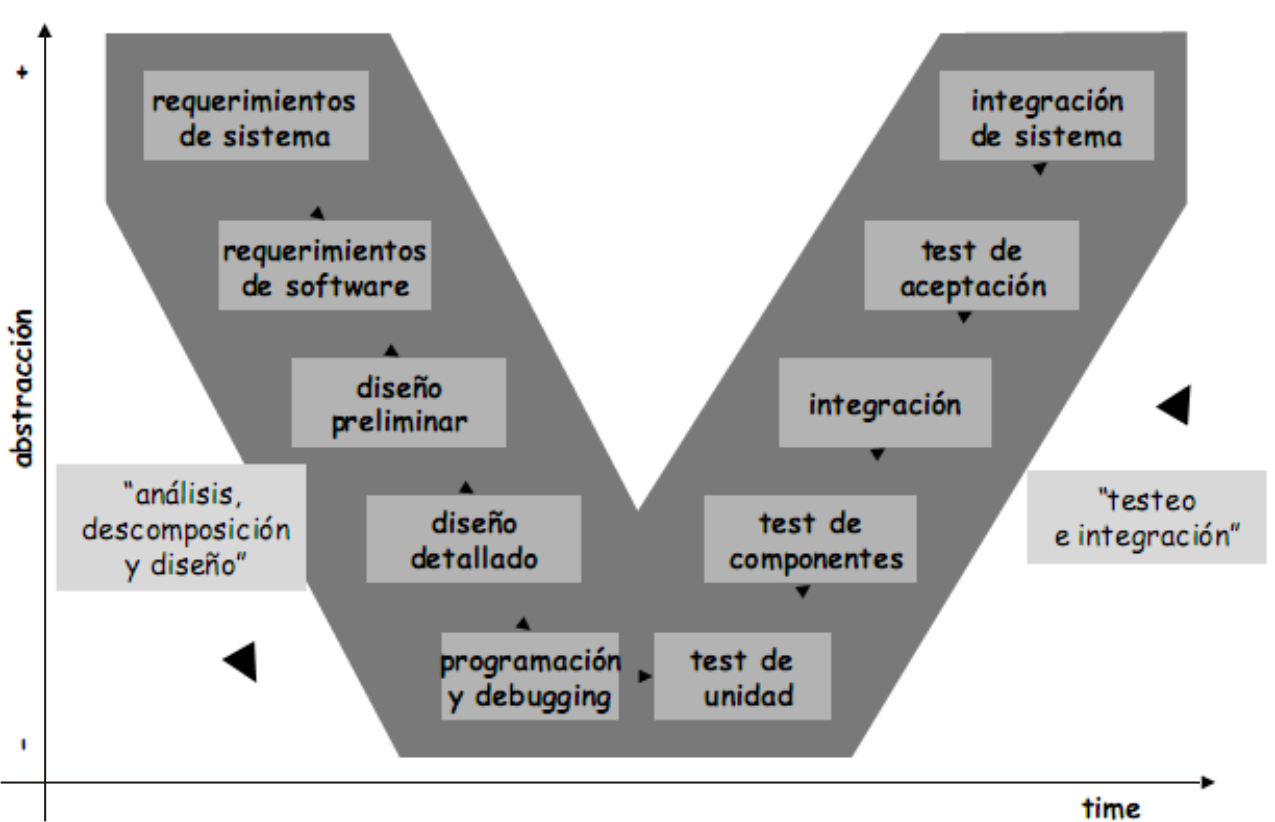
\includegraphics[width = 0.9\textwidth]{Graficos/ModeloV.png}

\subsection{Modelo Espiral (Boehm,1988)}

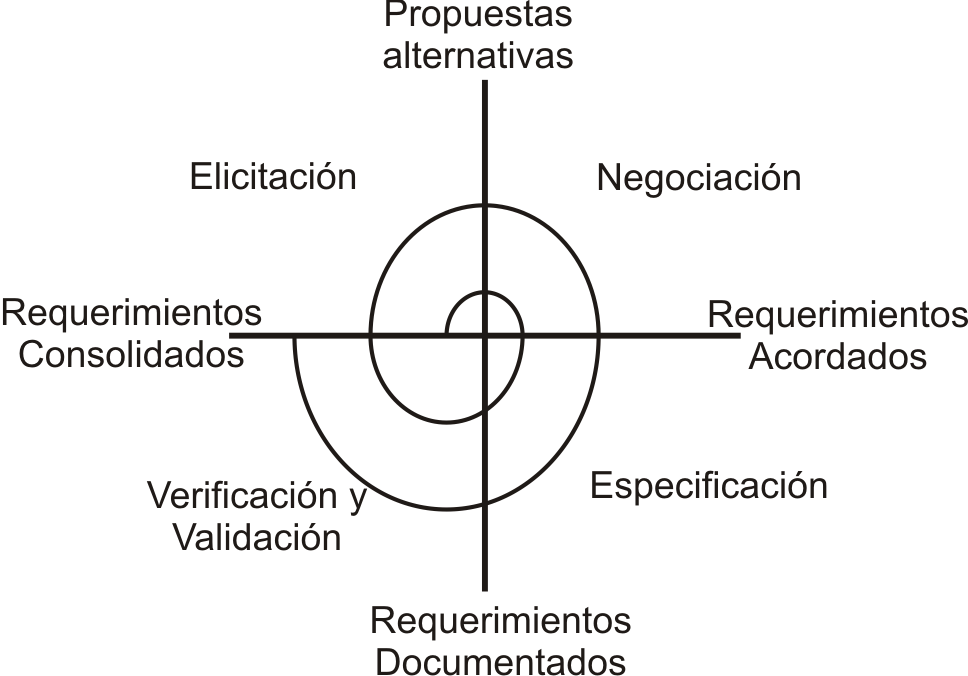
\includegraphics[width = 0.9\textwidth]{Graficos/ModeloEspiral.png}

\newpage

\subsection{Unified SW Development Process (Jacobson, 1999) }

Divisi�n en fases e iteraciones

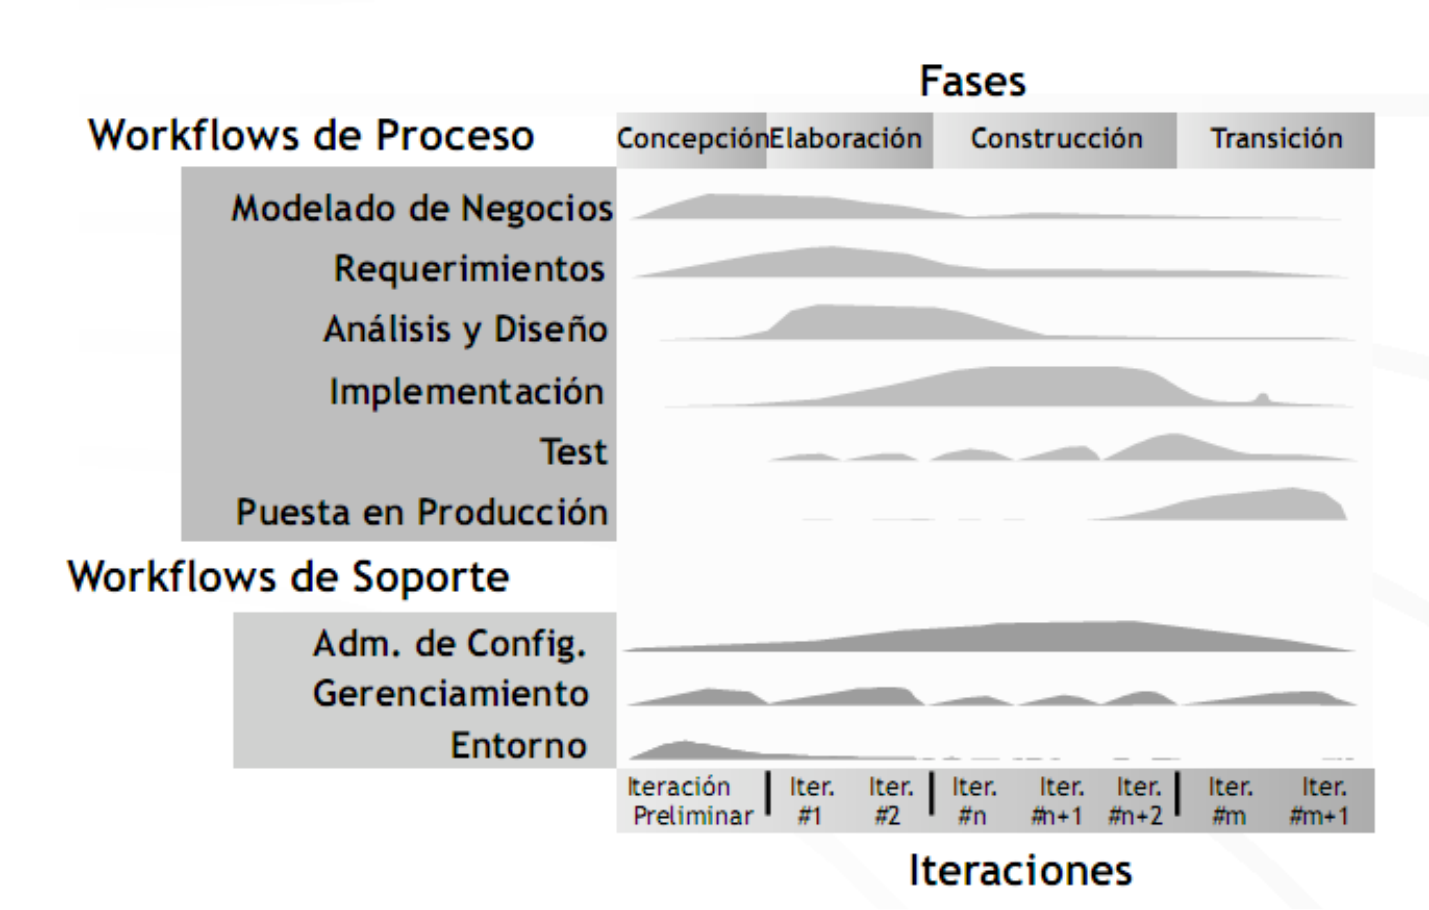
\includegraphics[width = 0.9\textwidth]{Graficos/ModeloJacobson.png}

\subsection{Modelo Twin Peaks}

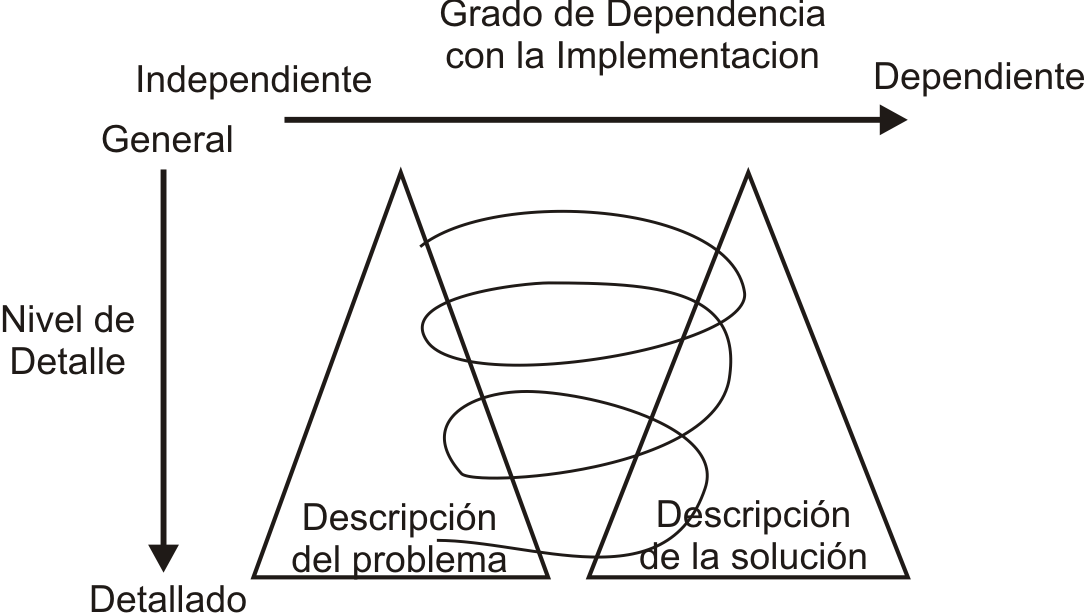
\includegraphics[width = 0.9\textwidth]{Graficos/ModeloTwinPeaks.png}

\newpage

\section{Modelos}

Un \emph{modelo} es una representaci�n de la realidad.

Los modelos son construidos con el objetivo de lidiar con la complejidad de los sistemas.

Los modelos son efectivos porque:

\begin{itemize}
	\item Describen un aspecto del problema a resolver
	\item Omiten detalles no relevantes al an�lisis para el cual se construye el modelo
	\item Permite comunicar en forma precisa aspectos del problema y la soluci�n a otras personas.
	\item Son m�s baratos de construir
	\item Facilita el an�lisis (permite detectar errores y falencias tempranamente)
\end{itemize}

Los modelos tienen un Scope y un Span

\begin{description}
	\item[Scope(aspecto):] tipo de fen�meno que se capta
	\item[Span(segmento):] individuos descriptos
\end{description}

\emph{Los modelos en Ingenier�a de Software son lenguajes formales con una denotaci�n precisa en el mundo real}


Los lenguajes formales tienen:

\begin{itemize}
	\item una \emph{sintaxis}(gr�fica/texto) para describirlos: cu�les son los garabatos permitidos
	\item una \emph{sem�ntica} para abstraer accidentes sint�cticos: cu�les de estos garabatos significan lo mismo.
\end{itemize}

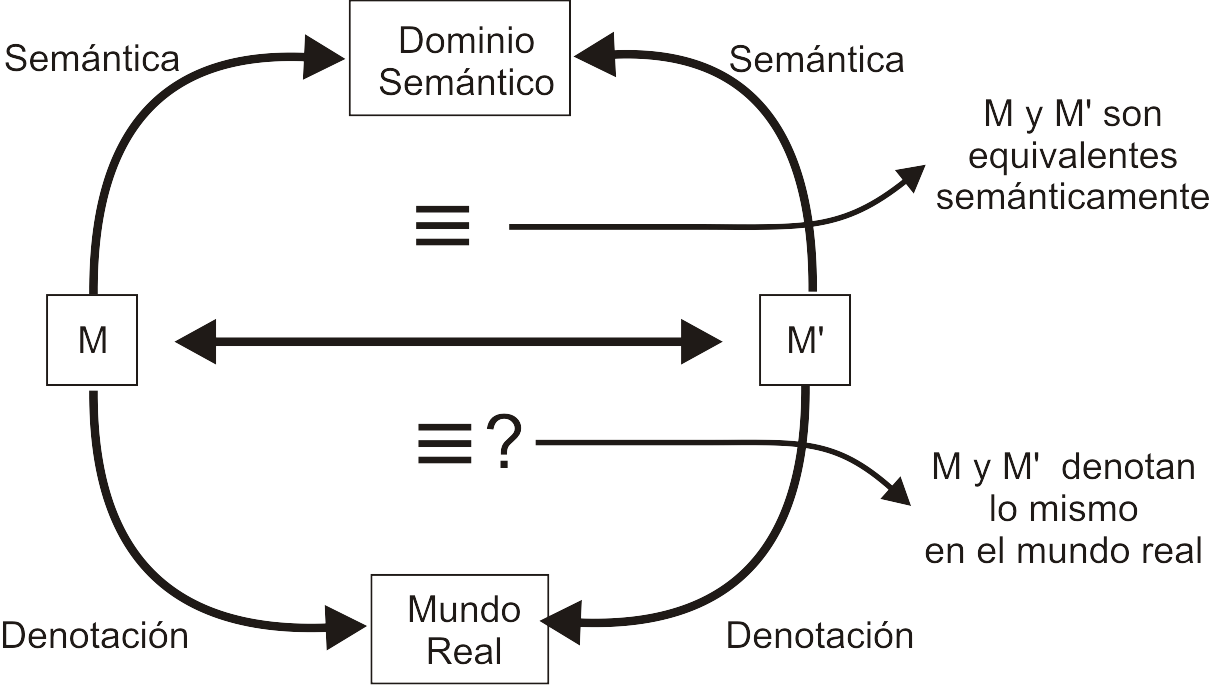
\includegraphics[width = 0.9\textwidth]{Graficos/Modelos.png}

Un sistema se analiza desde m�ltiples modelos complementarios. Cada modelos enfoca una aspecto(scope) del sistema, para permitir an�lisis rigurosos y escalables.

Es imposible vincular los distintos modelos formalmente, manteni�ndolos analizables y entendibles(�tiles).

Ejemplos de modelos: de Objetivos, de Agentes, de Operaciones, Conceptuales, de Comportamiento, Arquitect�nicos.

\newpage

\section{Validaci�n y Verificaci�n}
\label{VerificacionValidacion}
\begin{description}
	\item[Validaci�n:] $\longrightarrow$ Mundo vs. Modelo
	Proceso cuyo objetivo es \emph{incrementar la confianza} de que una descripci�n formal \emph{se corresponde} con la realidad. Es imposible de realizar.
	\item[Verificacion:] $\longrightarrow$ Modelo vs. Modelo
	Proceso cuyo objetivo es \emph{garantizar} que una descripci�n formal \emph{es correcta} con respecto a otra.
\end{description}

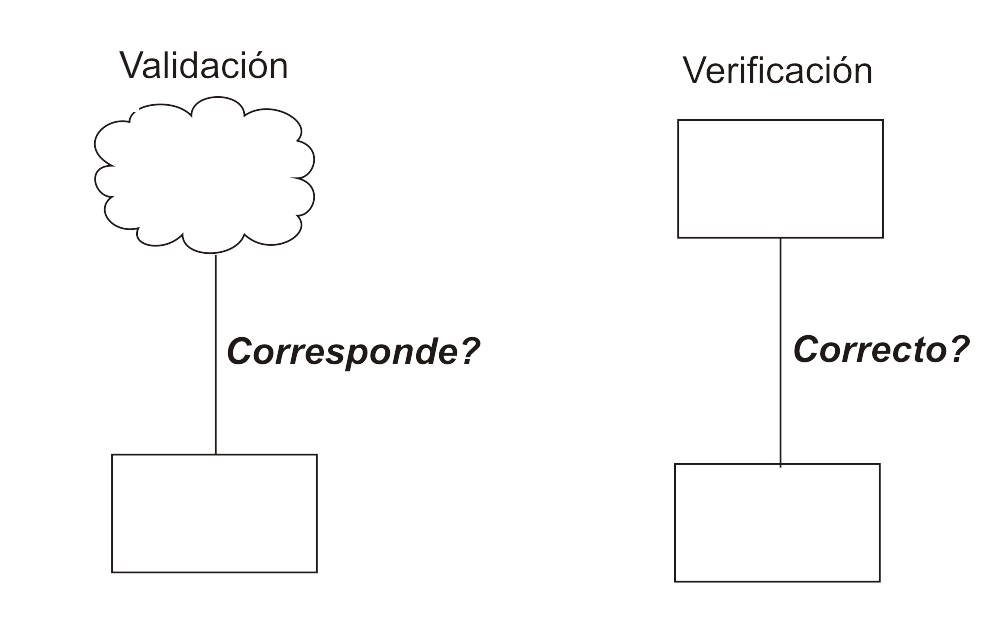
\includegraphics[width = 0.9\textwidth]{Graficos/VerificacionValidacion.png}

\section{Resumen}

\begin{itemize}
	\item Que es la IS? Definici�n, objetivos, problemas
	\item Ciclo de vida de desarrollo de Software
	\item Modelos: definici�n, ventajas	
		\begin{itemize}
			\item Scope y Span
			\item Sintaxis, Sem�ntica y Denotaci�n
			\item Verificaci�n y Validaci�n
		\end{itemize}
\end{itemize}